\documentclass{standalone}
\usepackage{pgfplots}
\pgfplotsset{compat=1.15,
    every axis/.append style={
            font=\large,
            line width=1pt,
            tick style={line width=0.8pt}}}

\begin{document}
\begin{tikzpicture}
\begin{axis}[
        xmin=1, xmax=10000, % x scale
        domain=0:10000,  % added, key improvements
]
\addplot    {1/(1e9*x/11.778*3.273e-8 - 3.273e-8 + 1)};
\addplot    coordinates{(.125, .744)};
\end{axis}

\end{tikzpicture}
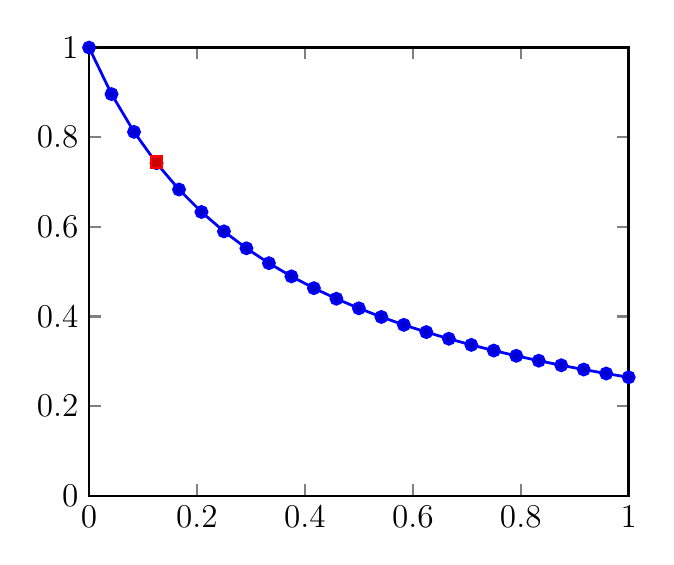
\begin{tikzpicture}
\begin{axis}[
        xmin=0, xmax=1, % x scale
        ymin=0, ymax=1, % y scale
        domain=0:1   % added, key improvements
]
\addplot    {1/((1e9*x/11.778)*3.273e-8-3.273e-8+1)};
\addplot    coordinates{(.125, .744)};
\end{axis}
\end{tikzpicture}

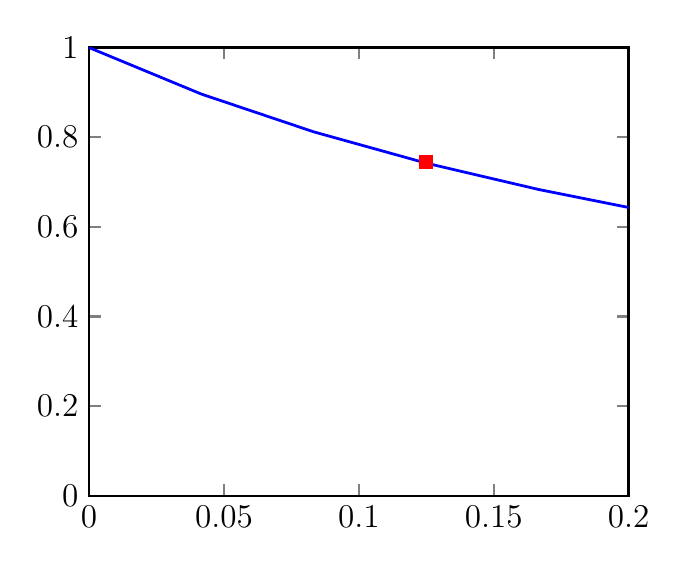
\begin{tikzpicture}
\begin{axis}[
        xmin=0, xmax=0.2, % x scale
        ymin=0, ymax=1, % y scale
        domain=0:1,% added, key improvements
        xticklabel style={/pgf/number format/.cd, fixed},% formattin ticks' labels
]
\addplot [blue,no marks]    {1/(1e9*x/11.778*3.273e-8 - 3.273e-8 + 1)};
\addplot [red,mark=square*] coordinates{(.125, .744)};
\end{axis}

\end{tikzpicture}
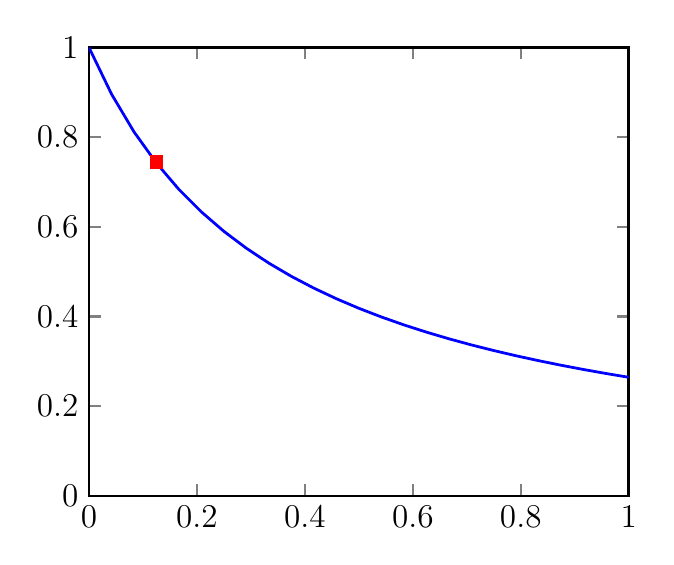
\begin{tikzpicture}
\begin{axis}[
        xmin=0, xmax=1, % x scale
        ymin=0, ymax=1, % y scale
        domain=0:1   % added, key improvements
]
\addplot [blue,no marks]    {1/((1e9*x/11.778)*3.273e-8-3.273e-8+1)};
\addplot [red,mark=square*] coordinates{(.125, .744)};
\end{axis}
\end{tikzpicture}

\end{document}